\documentclass{beamer}

\mode<presentation>
{
  \usetheme{Darmstadt}      % or try Darmstadt, Madrid, Warsaw, ...
  \usecolortheme{default} % or try albatross, beaver, crane, ...
  \usefonttheme{serif}  % or try serif, structurebold, ...
  \setbeamertemplate{navigation symbols}{}
  \setbeamertemplate{caption}[numbered]
} 
 
\usepackage[utf8]{inputenc}
\usepackage[]{algorithm2e}

%Information to be included in the title page:
\title{Nat-Sci II Presentation: \\
Editing of Pig DNA May Lead to More Organs for People}
\author{YD Choi, Amy Jung, Vaughn Tajirian, Katie Westerlund }
\institute{New York University}
 
\begin{document}
 
\frame{\titlepage} 

\begin{frame}
\frametitle{The Article under Investigation}
\begin{itemize} 
\item "Editing of Pig DNA May Lead to More Organs for People," appeared in
New York times Science section (10/15/15). Written by Carl Zimmer.
\end{itemize}
\begin{figure}[h!]
  \centering
    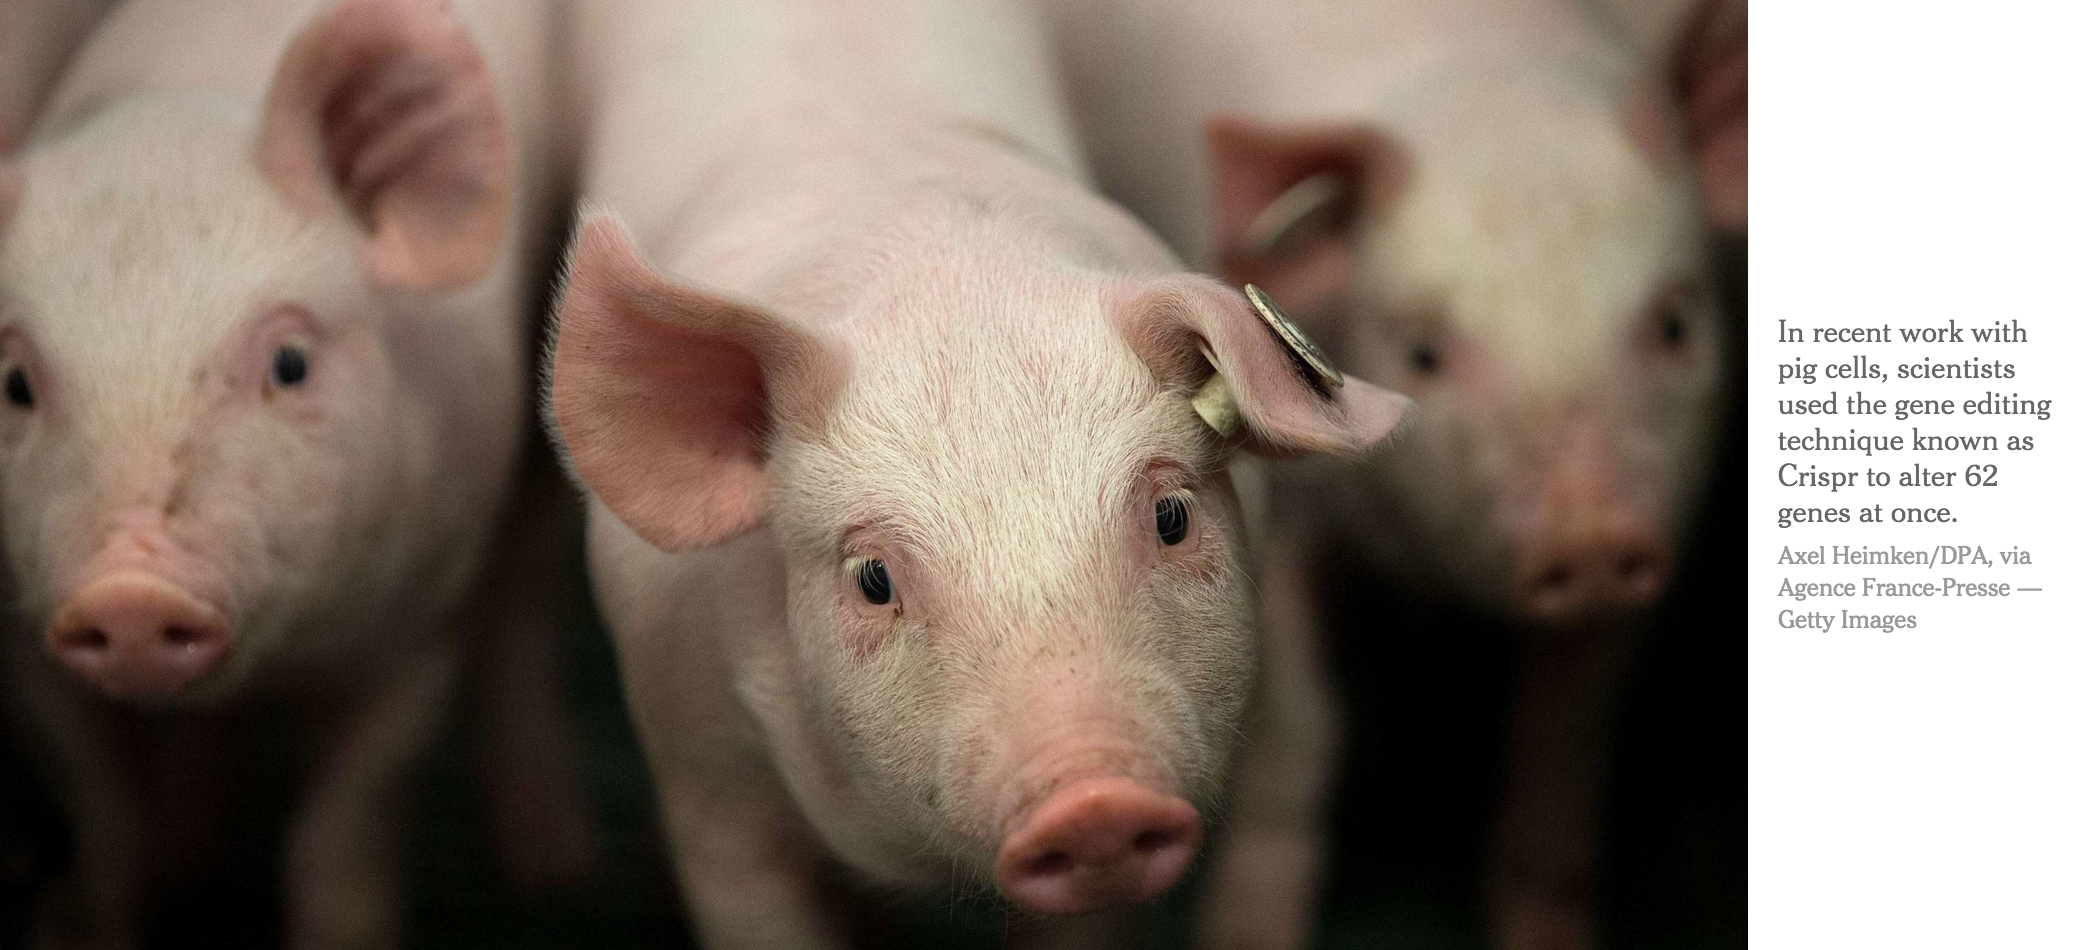
\includegraphics[width=1\textwidth]{edit-pigs.png}
\end{figure}
\end{frame}

\begin{frame}
\frametitle{CRISPR and Pigs' organs}
\end{frame}

\begin{frame}
\frametitle{What happened with CRISPR?}
\begin{itemize}
\item In October of 2015, scientists gathered at the National Academy of Sciences
in Washington to talk about Crispr, a new method for editing genes.
\item Carl Zimmer claims that "In the past couple of years, 
the technique has become so powerful and accessible that many experts are 
calling for limits on its potential uses — especially altering human 
embryos with changes that could be inherited by future generations."
\end{itemize}
\end{frame}
\begin{frame}
\frametitle{CRISPR: a new method for editing genes}
\begin{itemize}
\item 
CRISPRs (clustered regularly interspaced short palindromic repeats) are 
segments of prokaryotic DNA containing short repetitions of base sequences.
Each repetition is followed by short segments of "spacer DNA" from previous
exposures to a bacterial virus or plasmid.[2] It is pronounced "crisper" 
(Wikipedia).
\end{itemize}
\end{frame}


\begin{frame}
\frametitle{Recent development with CRISPR}
\begin{itemize}
\item "In a typical experiment, scientists use Crispr to alter a single gene.
 But in recent work with pig cells, Dr. Church and his colleagues used Crispr
 to alter 62 genes at once. The researchers hope that this achievement may
 someday make it possible to use pig organs for transplantation into humans." 
(Carl Zimmer) 
\item "But despite the large number of genes involved, 
Dr. Weiss and other experts cautioned that the 
new work doesn’t mean that we’ve suddenly gained the power to 
bypass evolution. Crispr does not allow scientists to manipulate 
genes on a huge scale — yet."

\end{itemize}
\end{frame}


\end{document}
